% The dvipsnames option is passed to the xcolor package, which beamer loads
\documentclass[xcolor={dvipsnames}]{beamer}

\usepackage{smpa2152-style}

\title[Predictive Election Models]{Predictive Election Models}
\author[SMPA 2152]{Data Analysis for Journalism and Political Communication (Spring 2025)}
\date{Prof. Bell}

\begin{document}

%%%%%%%%%%%%%%%%%%%%%%%%%%%%%%%%%%%%%%%%%%%%%%%%%%%%%%%%%%%%%%%%%%
\frame{
\titlepage
}

%%%%%%%%%%%%%%%%%%%%%%%%%%%%%%%%%%%%%%%%%%%%%%%%%%%%%%%%%%%%%%%%%%
\frame{\frametitle{Dart-Throwing Chimpanzees}

\centering
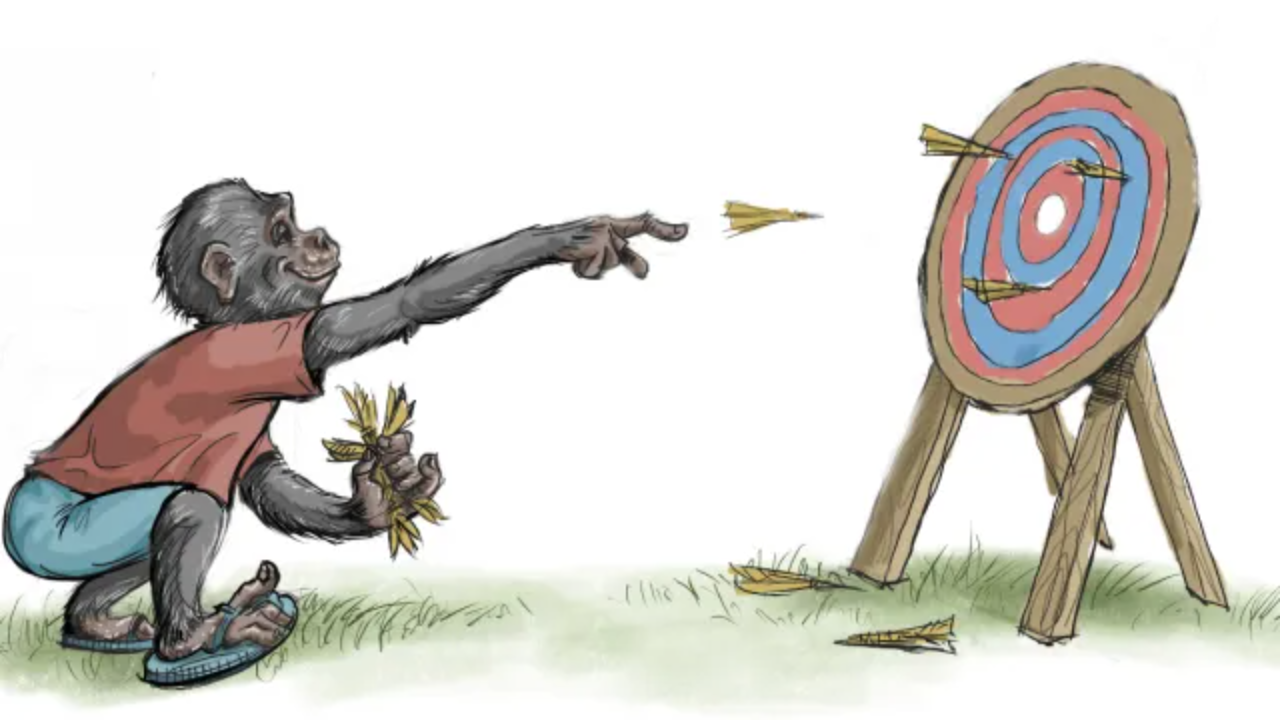
\includegraphics[width = .8\textwidth]{dart_throwing_chimps.png}
}

%%%%%%%%%%%%%%%%%%%%%%%%%%%%%%%%%%%%%%%%%%%%%%%%%%%%%%%%%%%%%%%%%%
\frame{\frametitle{Expert Political Judgment}

\centering
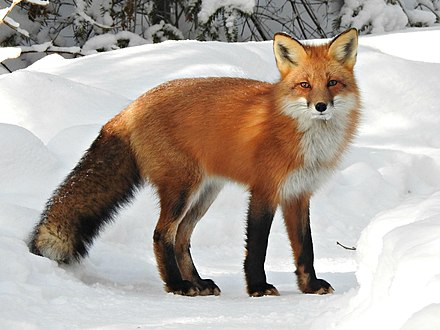
\includegraphics[width = .4\textwidth]{fox.jpg}
\hspace{2pt} vs. \hspace{2pt}
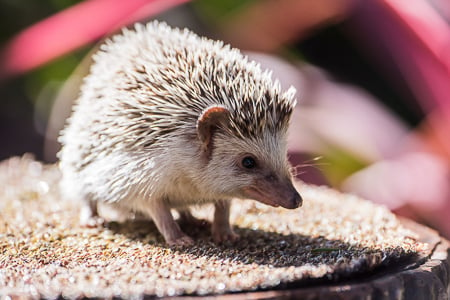
\includegraphics[width = .45\textwidth]{hedgehog.jpg}
}

%%%%%%%%%%%%%%%%%%%%%%%%%%%%%%%%%%%%%%%%%%%%%%%%%%%%%%%%%%%%%%%%%%
\frame{\frametitle{Wisdom of the Crowds}

\only<1>{
    \centering
    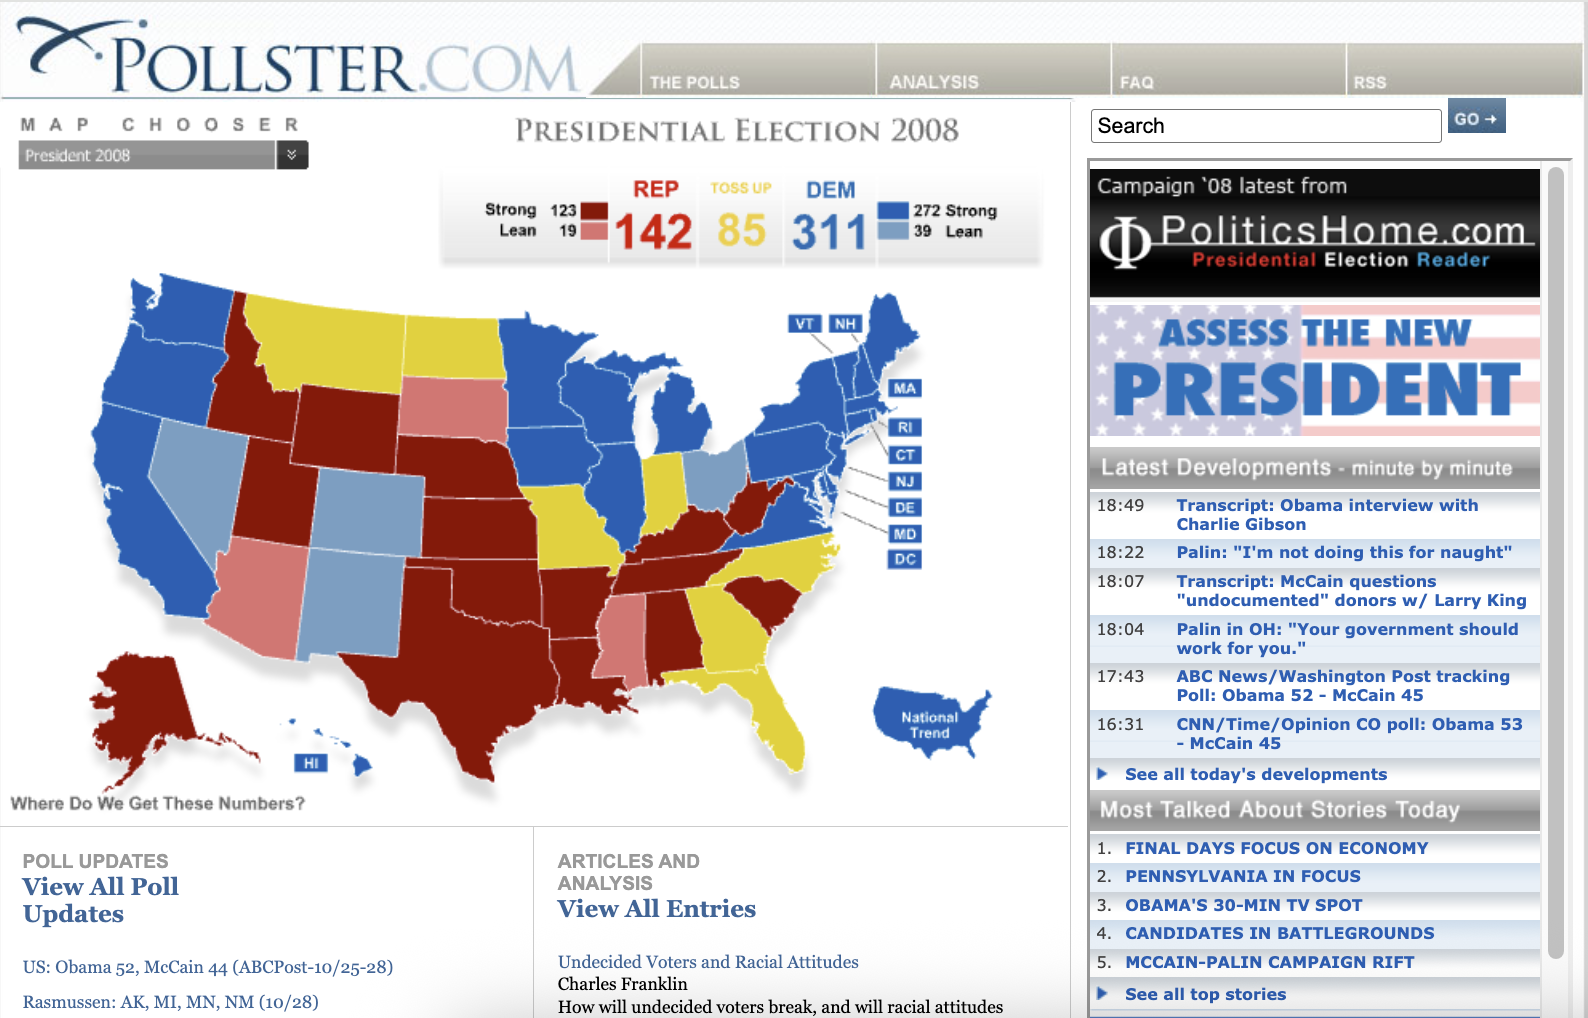
\includegraphics[width = .9\textwidth]{pollster_oct_29_2008.png}
}

\only<2>{
    \centering
    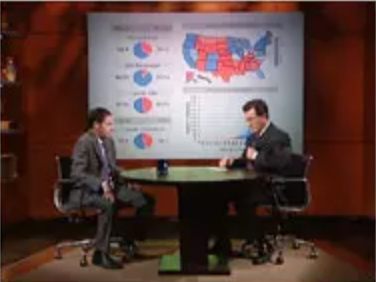
\includegraphics[height = .5\textheight]{silver_colbert.png}
}

\only<3>{
    \centering
    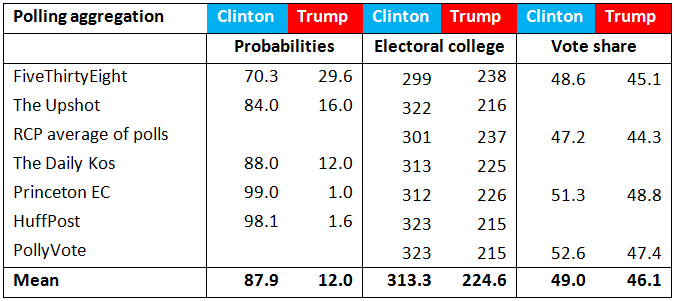
\includegraphics[width = .9\textwidth]{2016_predictions.png}
}

\only<4>{
    \centering
    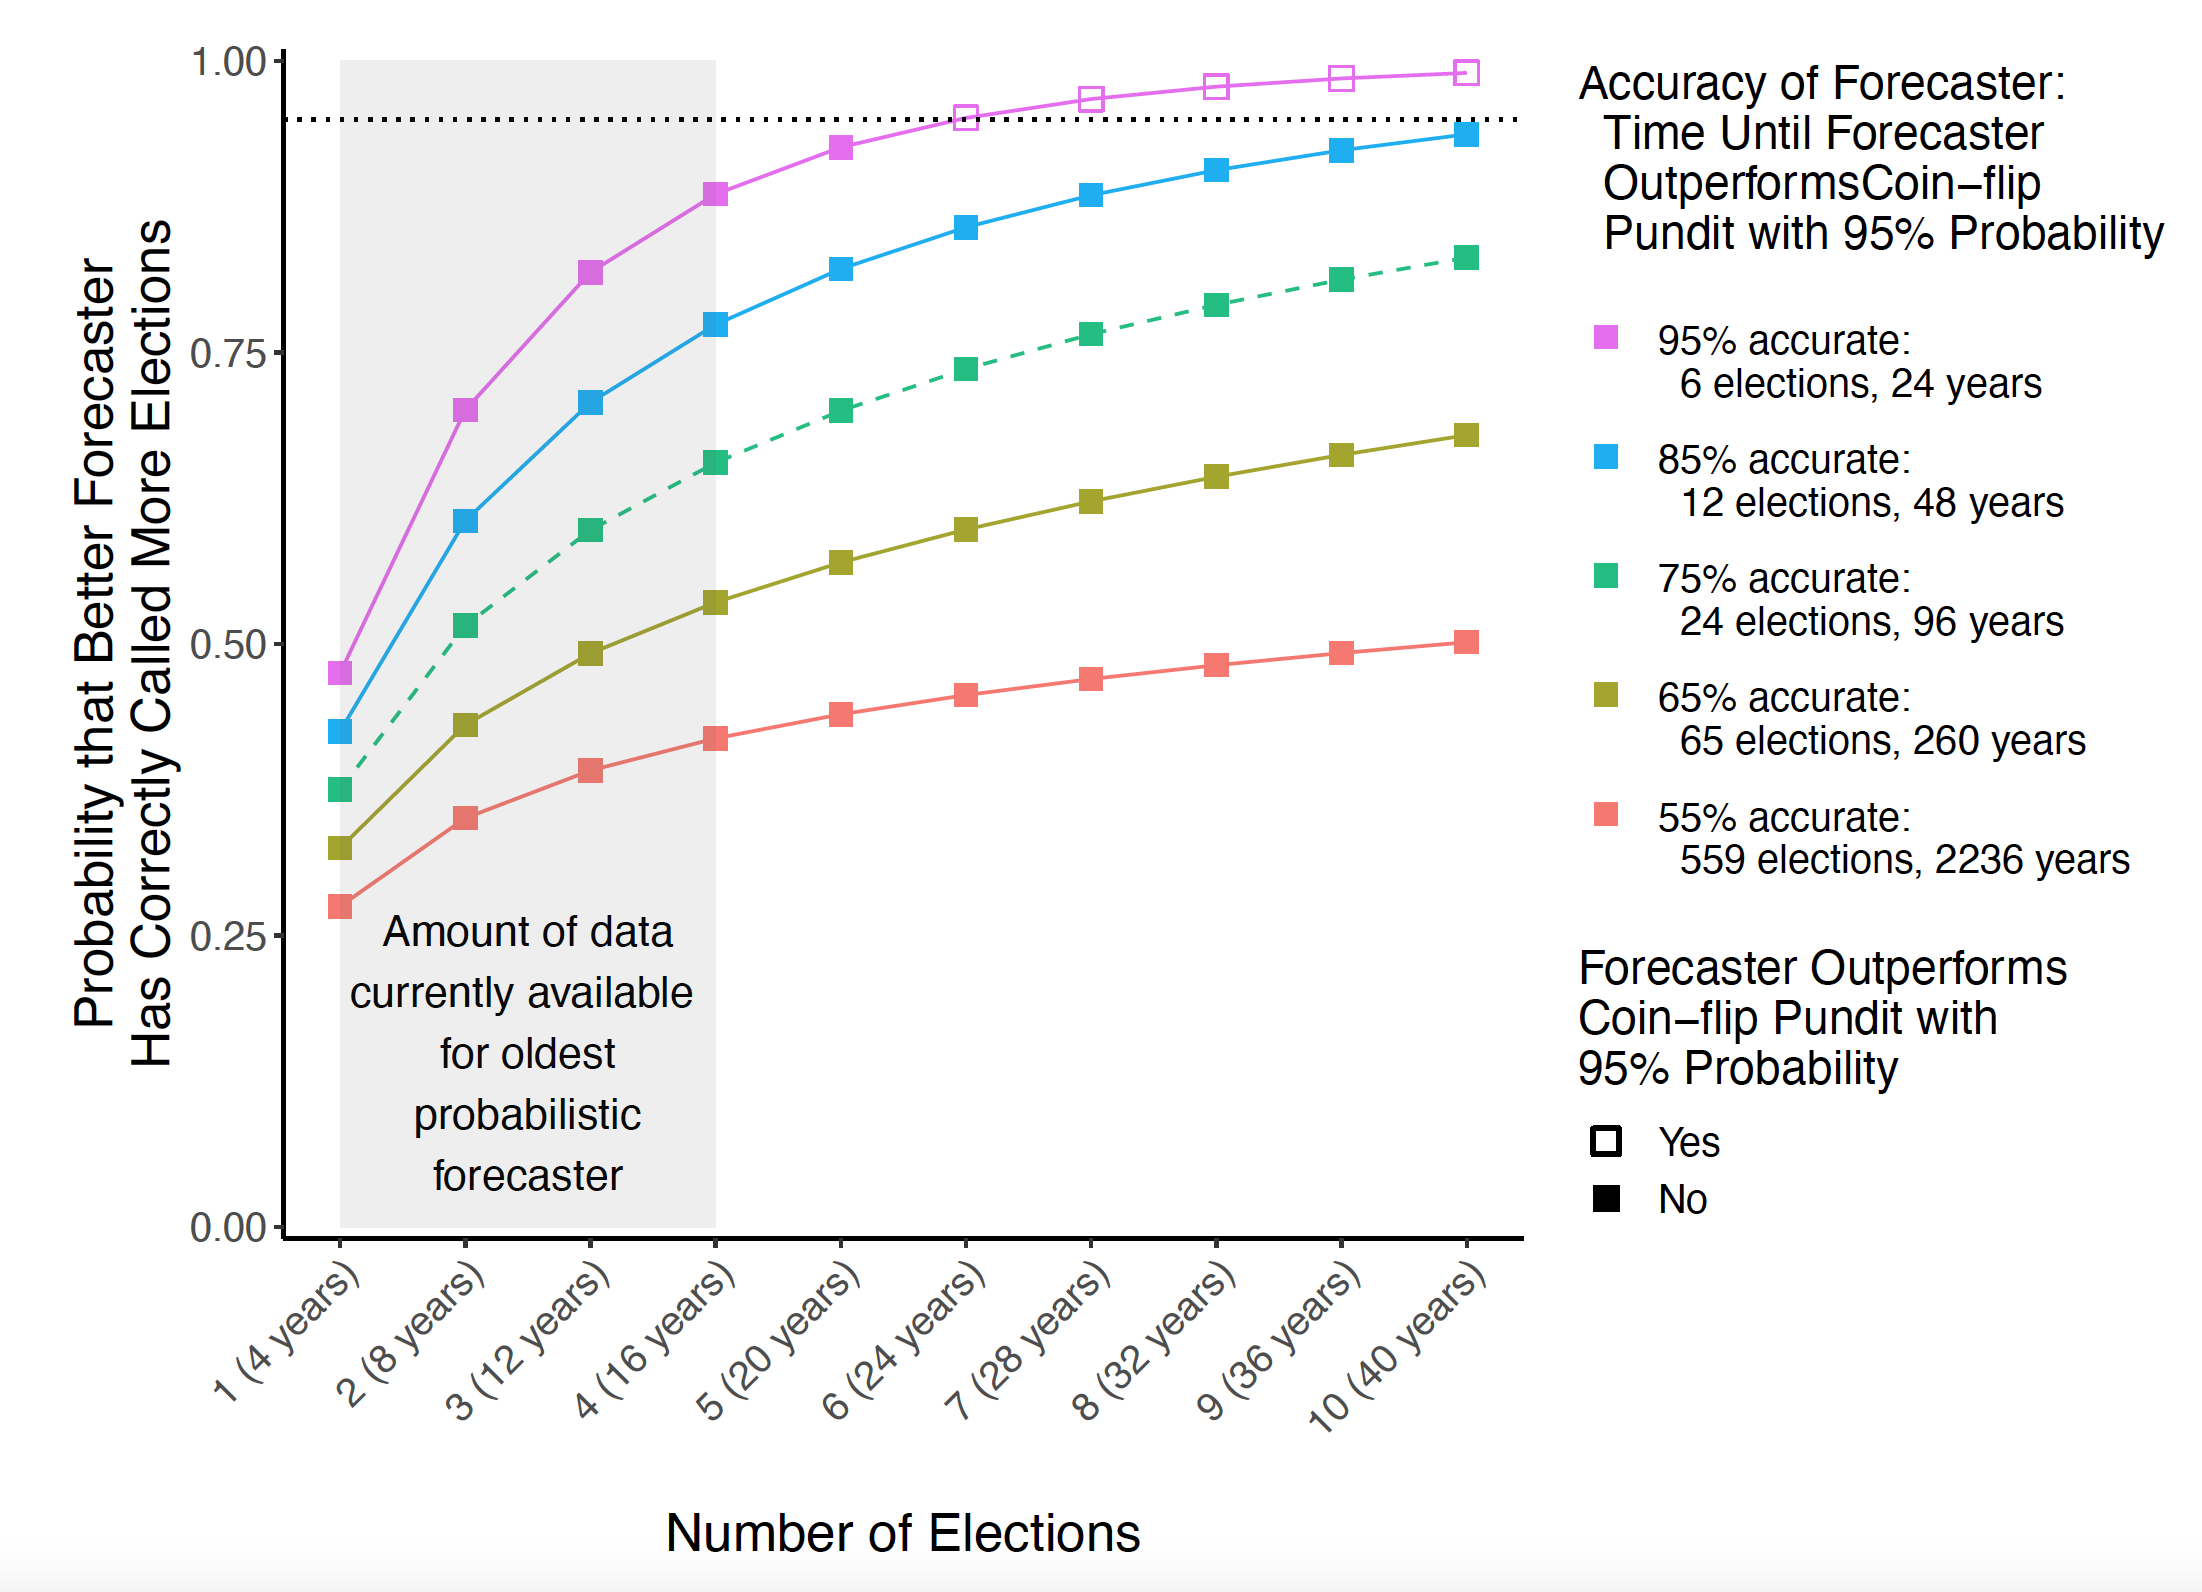
\includegraphics[width = .8\textwidth]{forecasting_accuracy.png} \\
    \tiny Source: Grimmer, Justin, Dean Knox, and Sean Westwood. 2024. ``Assessing the Reliability of Probabilistic US Presidential Election Forecasts May Take Decades.'' OSF Preprints. August 26. doi:10.31219/osf.io/6g5zq.
}

\only<5>{
    \centering
    \hspace{2em}
    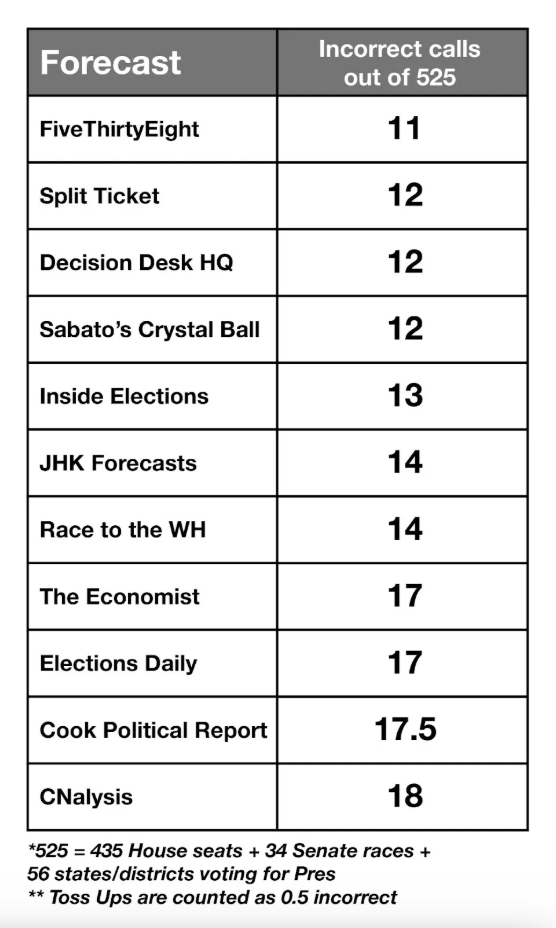
\includegraphics[width = .35\textwidth]{split_ticket_2024_performance_1.png}
    \hfill
    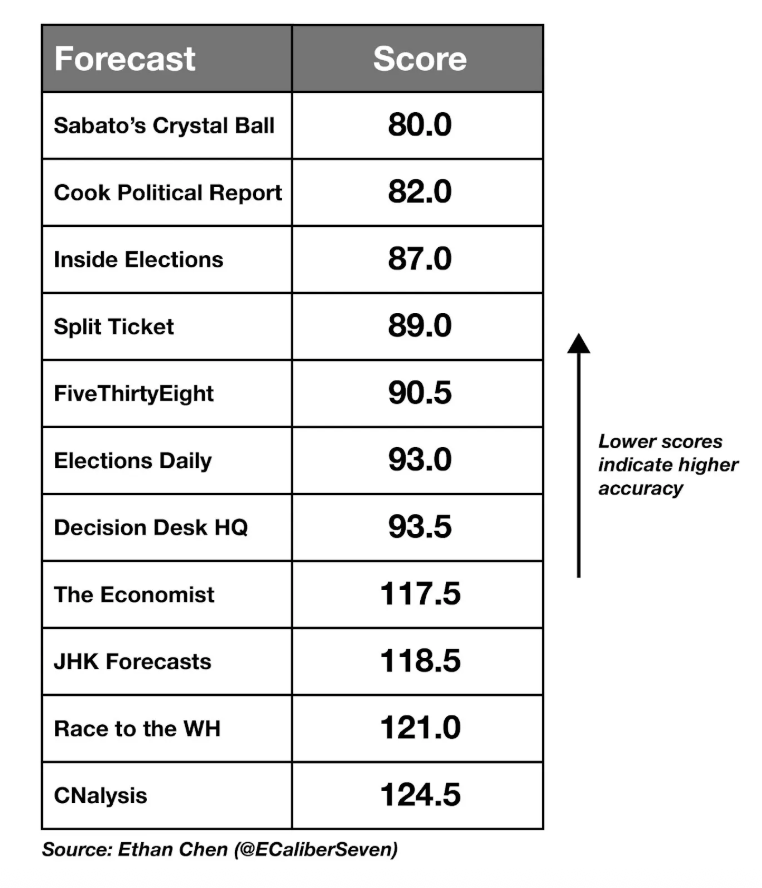
\includegraphics[width = .5\textwidth]{split_ticket_2024_performance_2.png}
}
}

%%%%%%%%%%%%%%%%%%%%%%%%%%%%%%%%%%%%%%%%%%%%%%%%%%%%%%%%%%%%%%%%%%
\frame{\frametitle{How Prediction Models Work}

\only<1>{
    \centering
    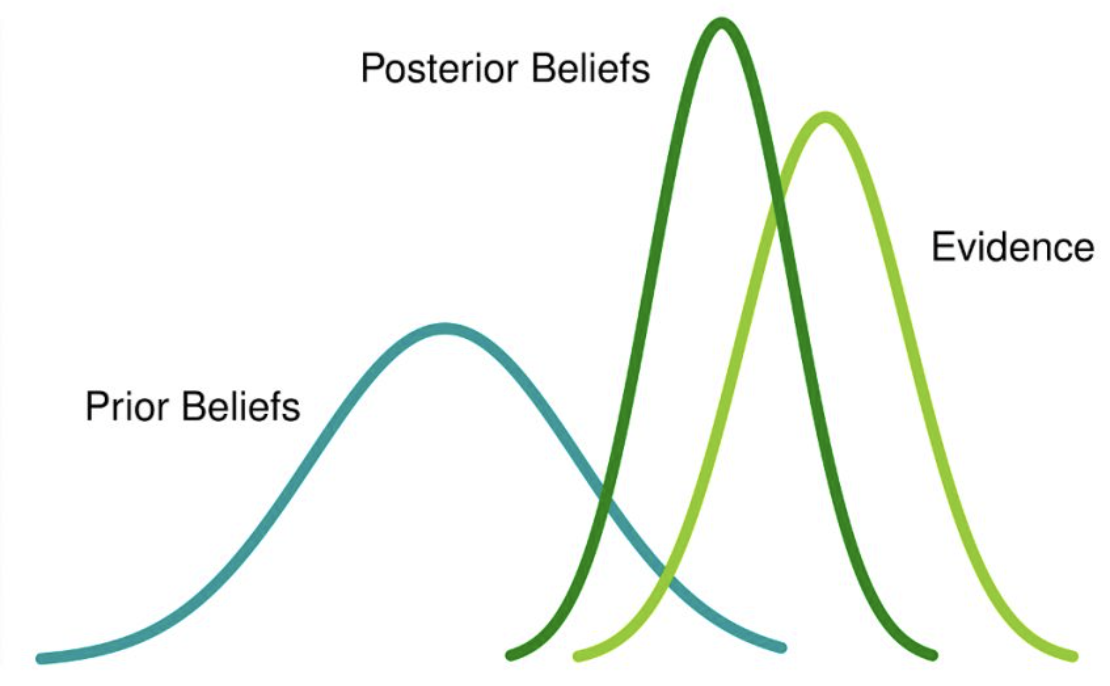
\includegraphics[width = .8\textwidth]{bayesian.png}
}

\only<2>{
    \centering
    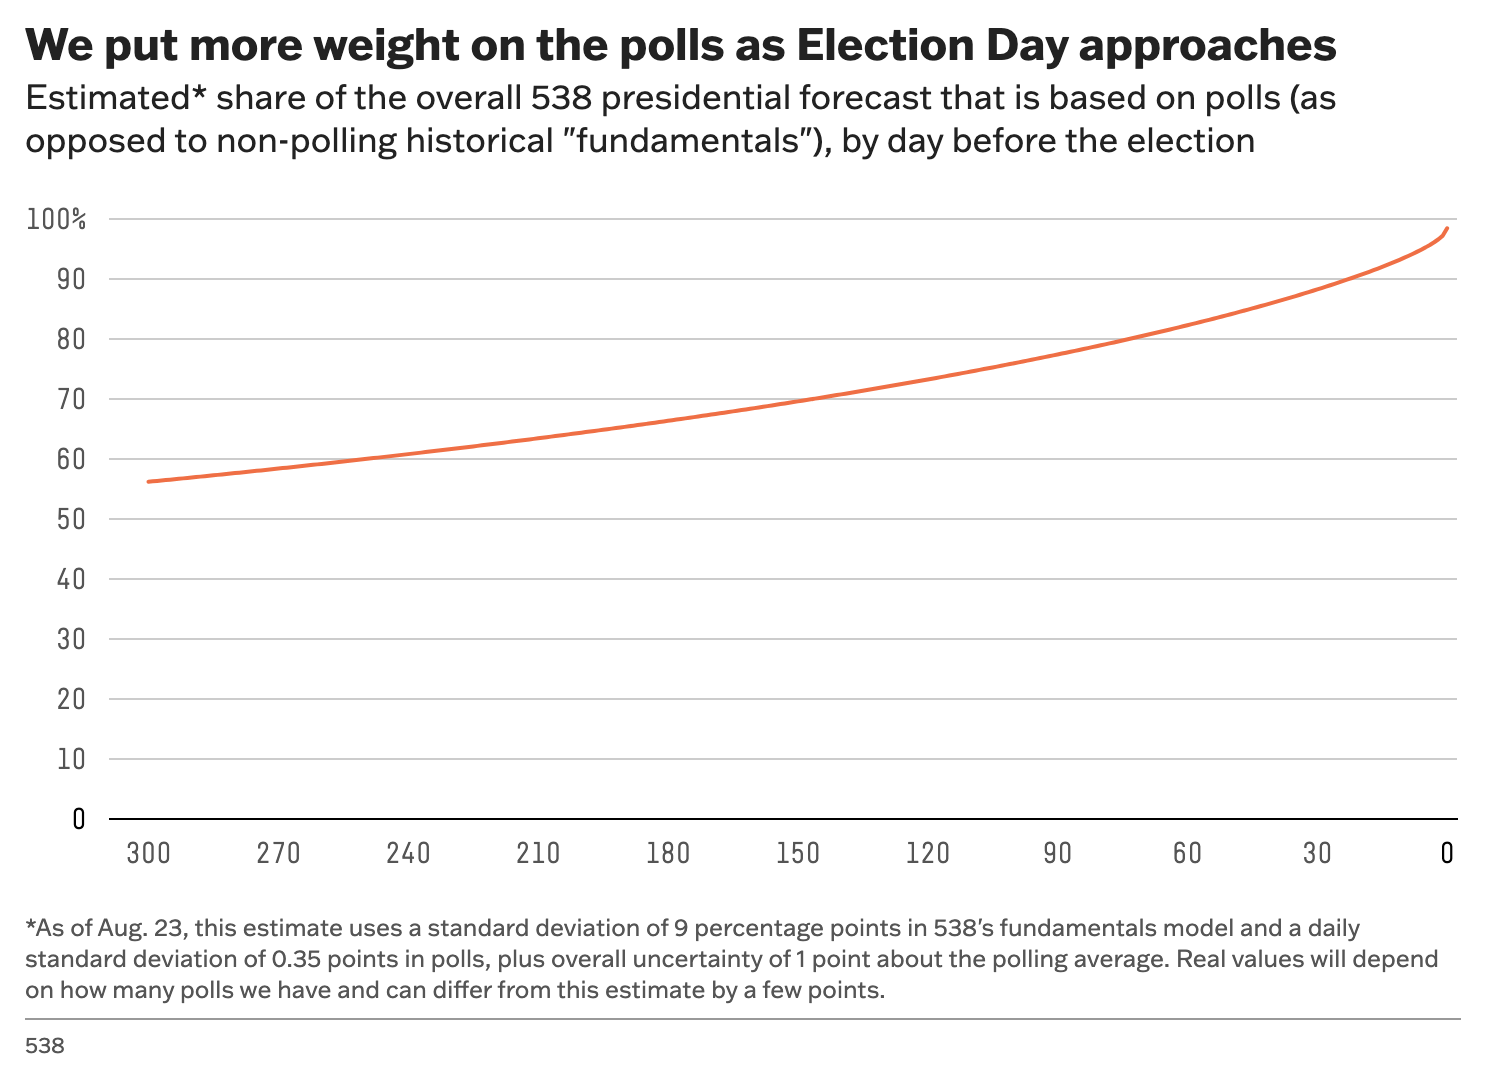
\includegraphics[width = .8\textwidth]{fundamentals_decay.png}
}

\only<3-5, 7-8>{
Election prediction models must decide:
    \begin{itemize}[<+(2)->]
        \item What polls to include (and how much to weight them): quality, quantity, sample size, time, etc.
        \item How to adjust polls for house effects and/or mode effects
        \item How to quantify the uncertainty in poll results
        \item<7-> How to model election outcomes (e.g, intra-state correlation)
        \item<8-> How to communicate probabilities
    \end{itemize}
}

\only<6>{
    \centering
    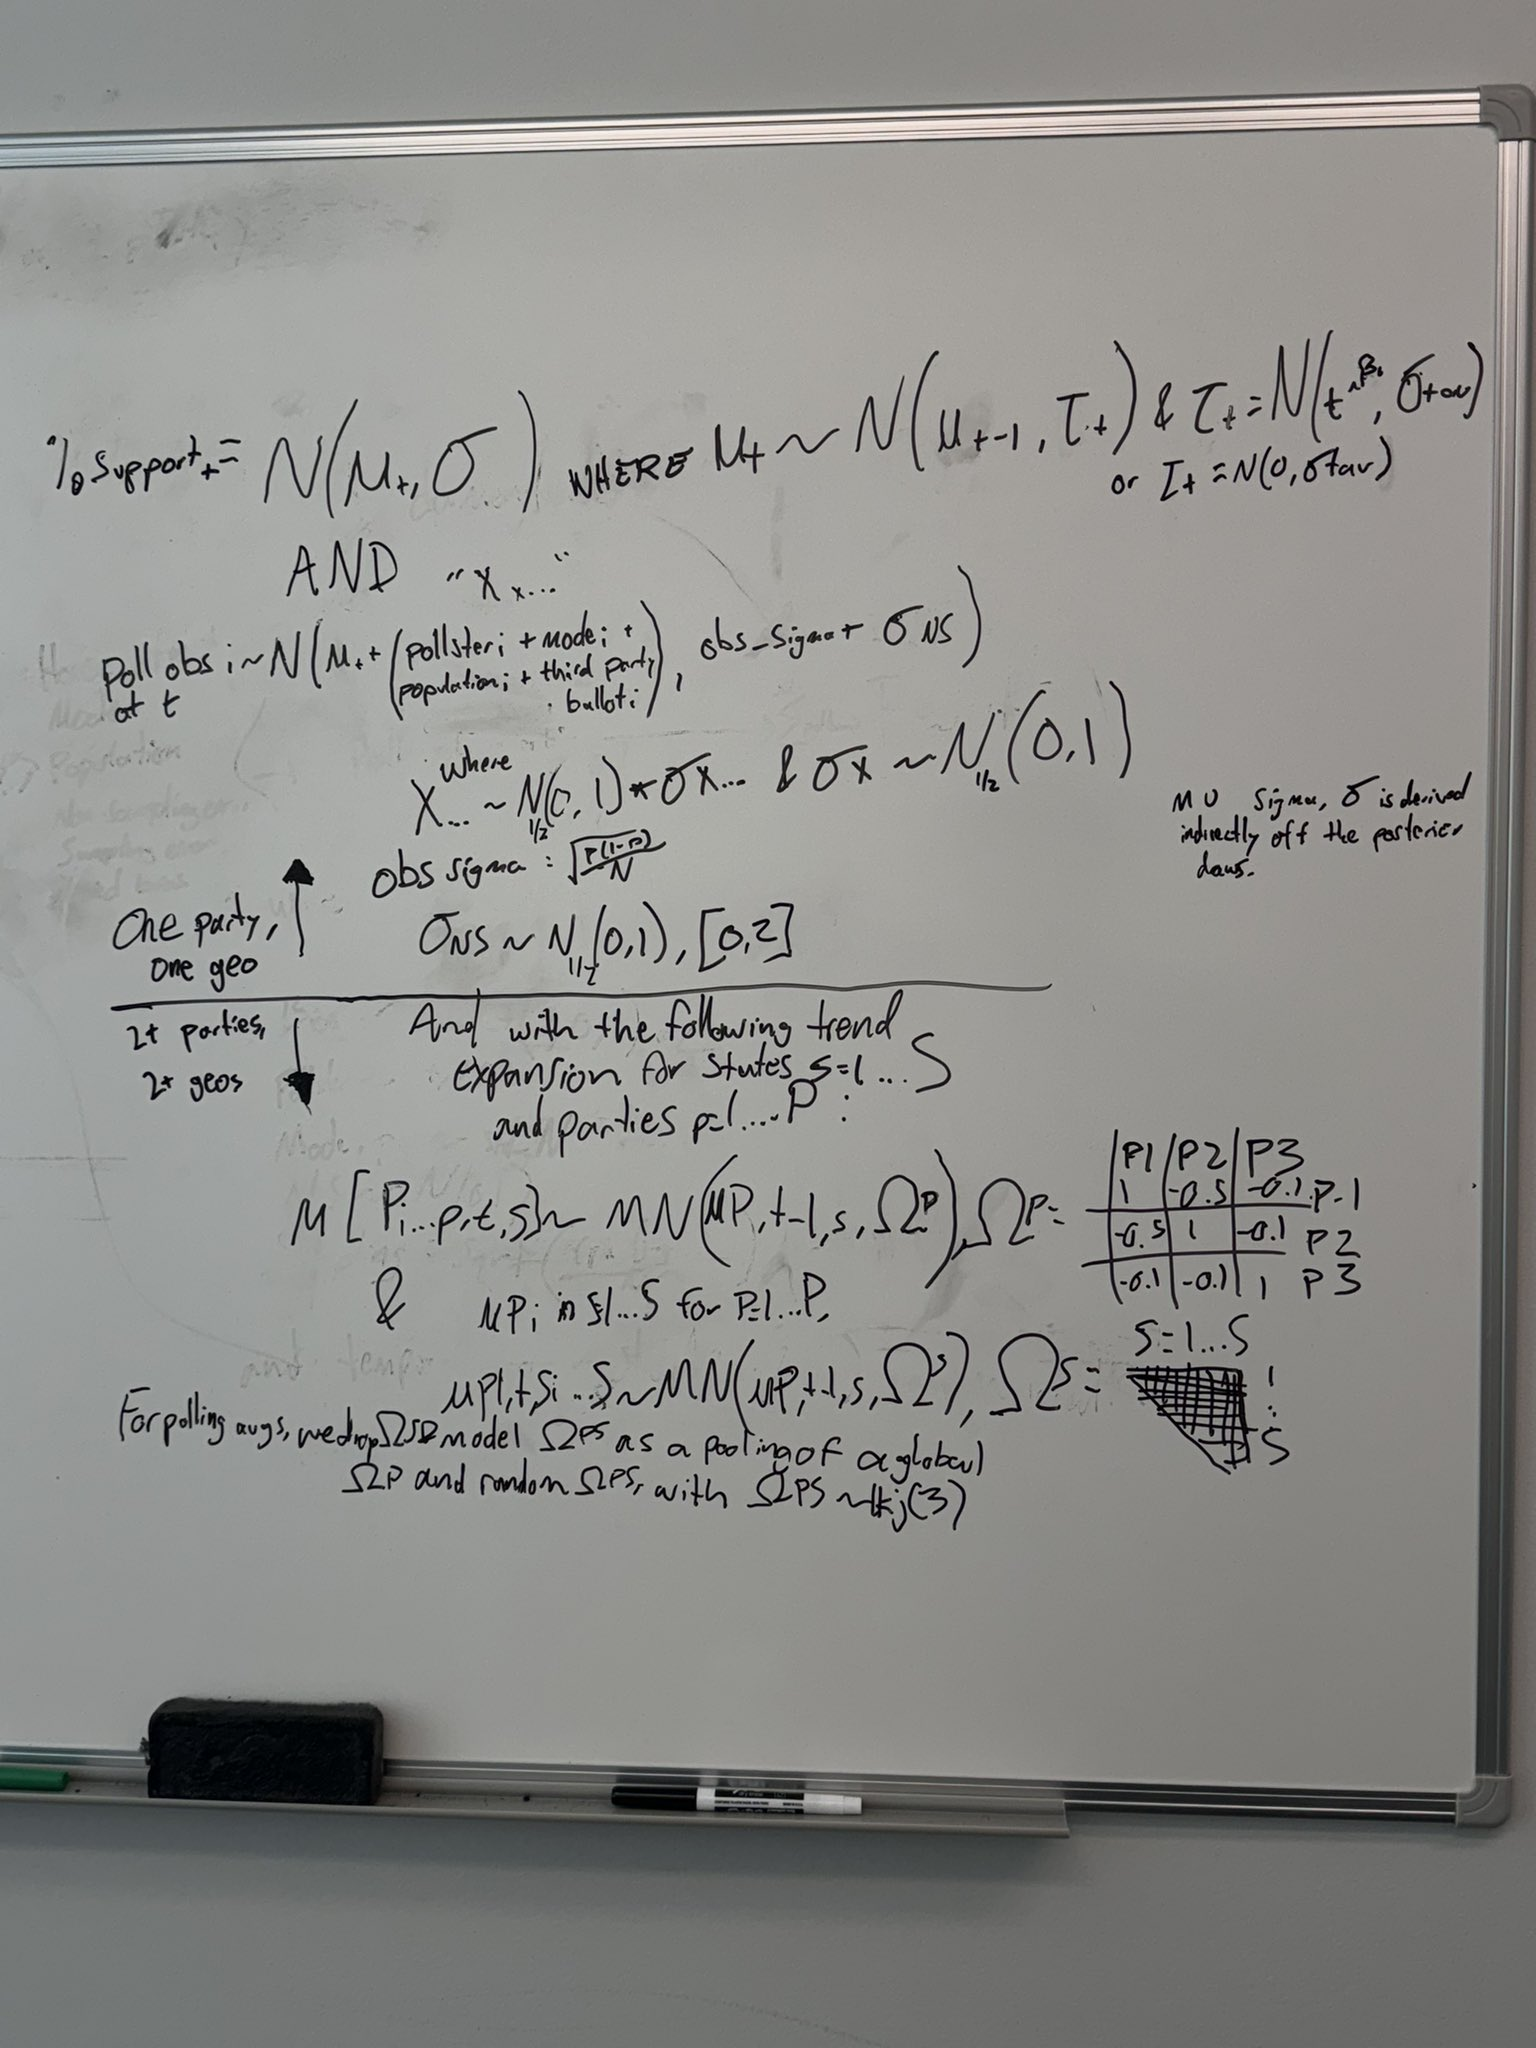
\includegraphics[height = .8\textheight]{morris_economist_whiteboard.jpeg}
}

}

%%%%%%%%%%%%%%%%%%%%%%%%%%%%%%%%%%%%%%%%%%%%%%%%%%%%%%%%%%%%%%%%%%
\frame{\frametitle{Next Frontiers}
\only<1,3-4,6>{
    \begin{itemize}[<+->]
        \item New sources of data (e.g., social media behavior)
        \item<3-> AI digital personas
        \item<4-> Prediction markets
        \item<6-> Do complex models outperform the fundamentals?
    \end{itemize}
    }

\only<2>{
    \centering
    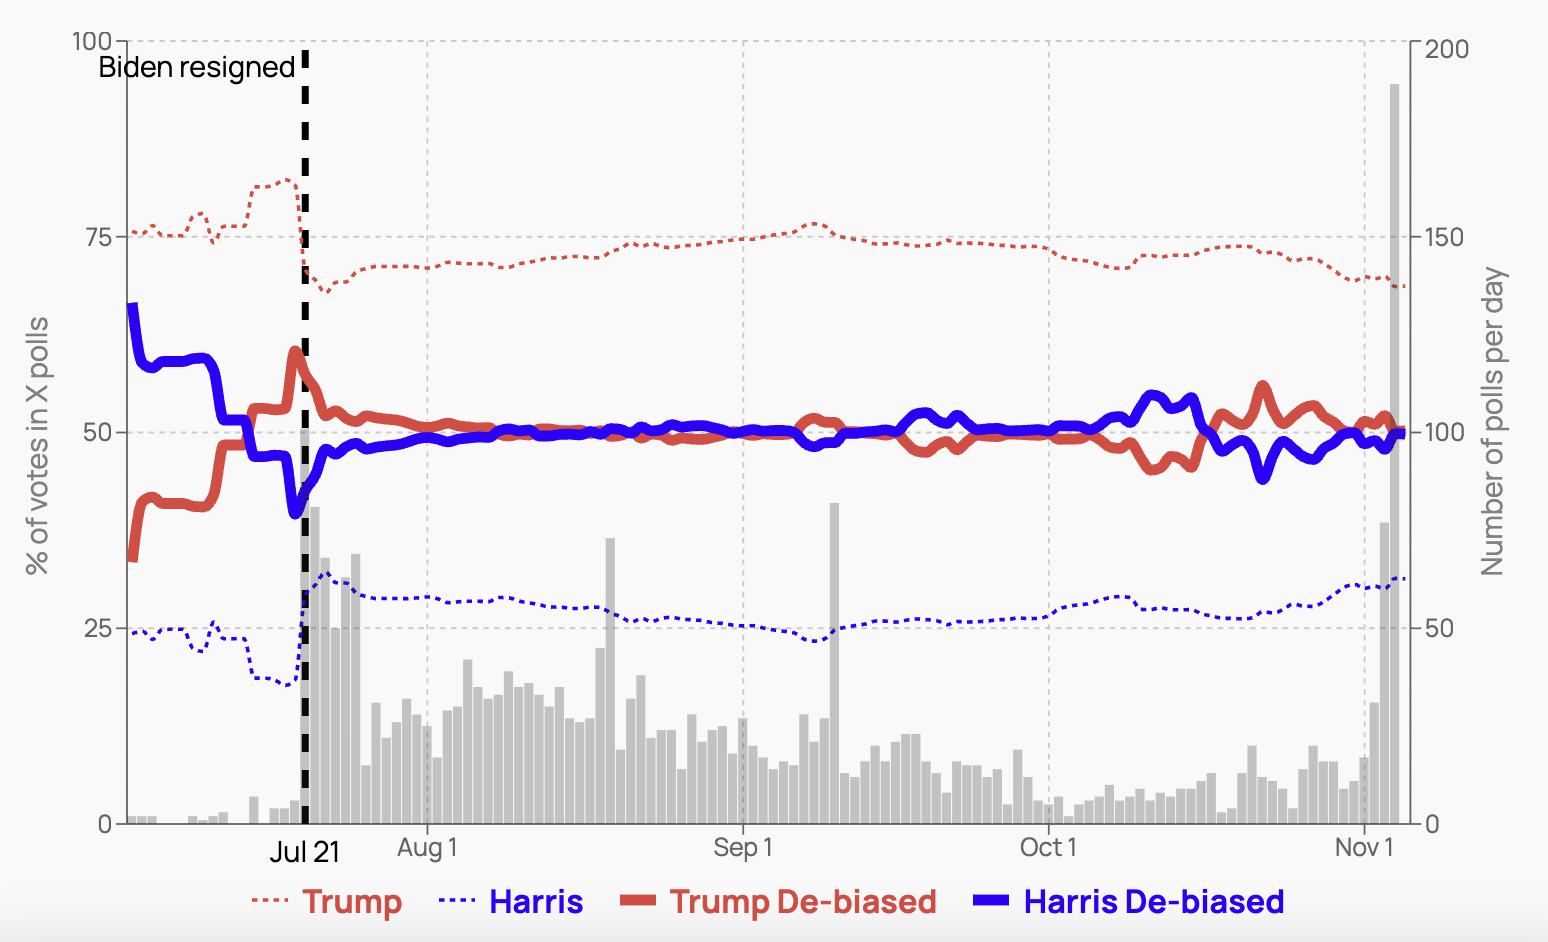
\includegraphics[width = .9\textwidth]{social_polls.png}
}

\only<5>{
    \centering
    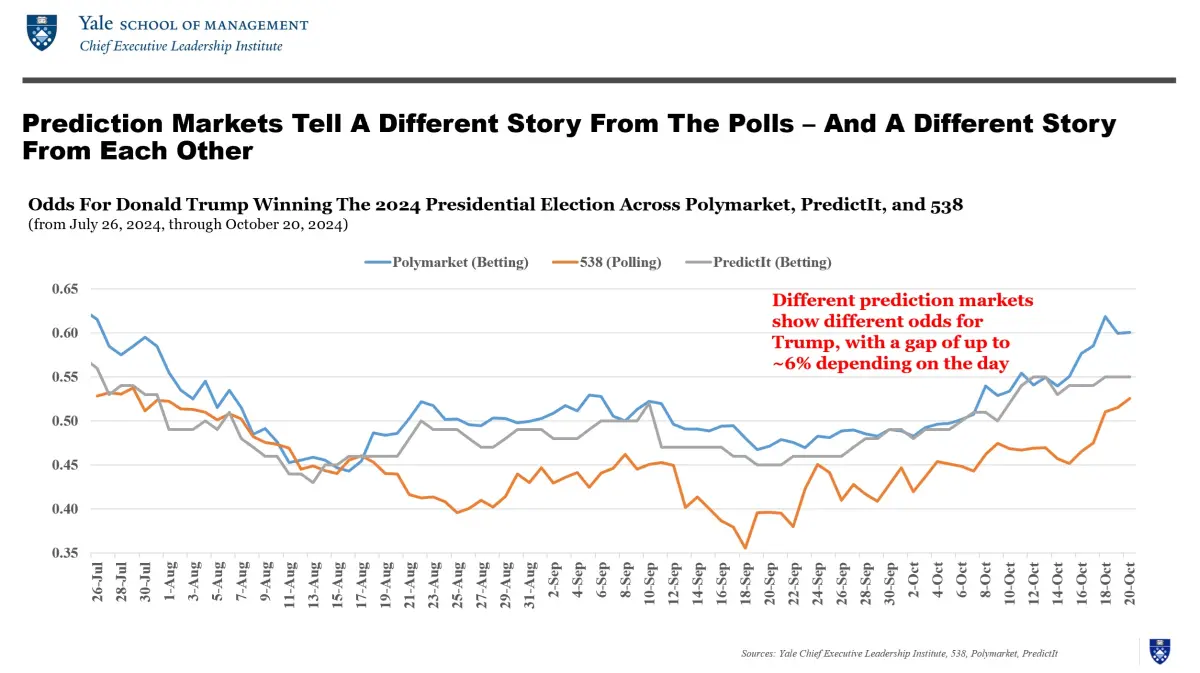
\includegraphics[width = .9\textwidth]{2024_prediction_markets.png}
}
    
}

\end{document}
